\documentclass[article.tex]{subfiles}
\begin{document}

In this section we will show how different boundary condition can be
used to construct interesting patterns on the studied facades. We start
with a discrete conformal map of the doubly-curved model to a standard
cylinder. The target angles have to be set to $\pi$ for all boundary
vertices to construct such a map. The result is shown in
Figure~\ref{fig:dc_cylinder}.

\begin{figure}[tb]
  \centering
  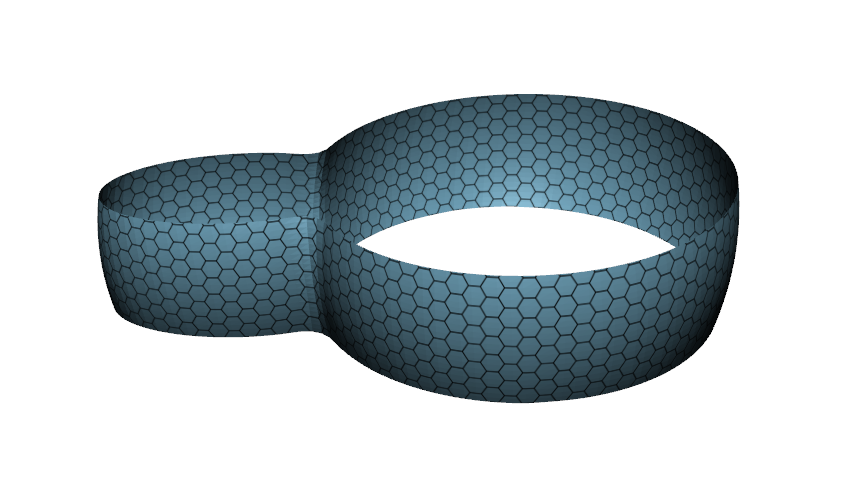
\includegraphics[width=.49\linewidth]{images/dc_cylinder_model_hex.png}
  \hfill
  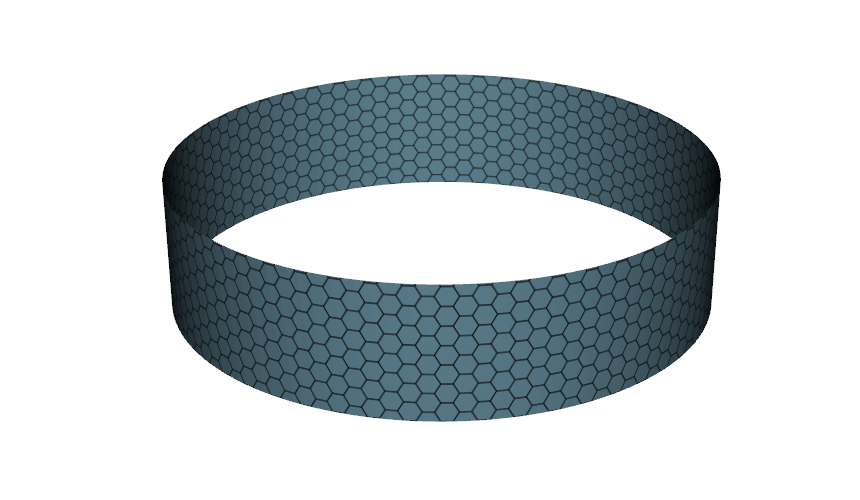
\includegraphics[width=.49\linewidth]{images/dc_cylinder_map_hex.png}
  \caption{A discrete conformal map from a doubly curved facade onto a
    standard cylinder.}
  \label{fig:dc_cylinder}
\end{figure}

Such a map can be used as a starting point to obtain a tesselation
with equal hexagons as described in
Section~\ref{sec:regular_hexagons}.

It is also possible to specify more exciting boundary condition: If
one aims for a panelization with boundary aligned hexagons or
triangles, then the boundary angles specified should be multiples of
$\tfrac{\pi}{3}$ (in case of quadrilaterals multiples of
$\tfrac{\pi}{4}$). A triangle example with two boundary vertices with
angles $\frac{4}{3}\pi$ and one with $\tfrac{\pi}{3}$ is shown in
Figure~\ref{fig:entrance}. The unrolled image shows the specified
angles, that are $\pi$ for all other vertices. At the vertices with
angle~$\tfrac{4}{3}\pi$ the lower boundary ``bends'' inside around the
vertex with angle~$\tfrac{\pi}{3}$.

\begin{figure}[b]
  \centering
  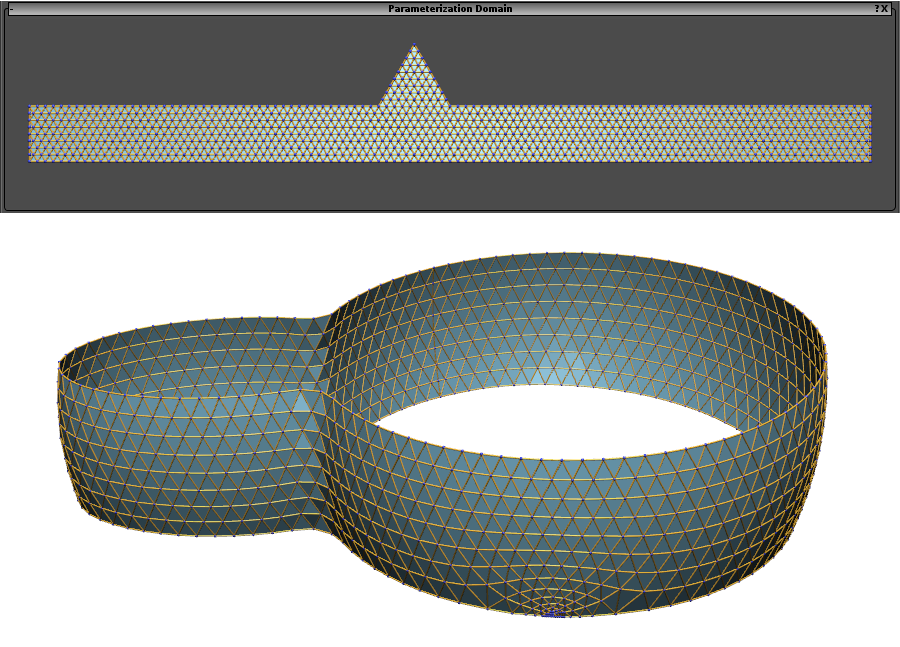
\includegraphics[width=.49\linewidth]{images/dc_entrance_map.png}
  \hfill
  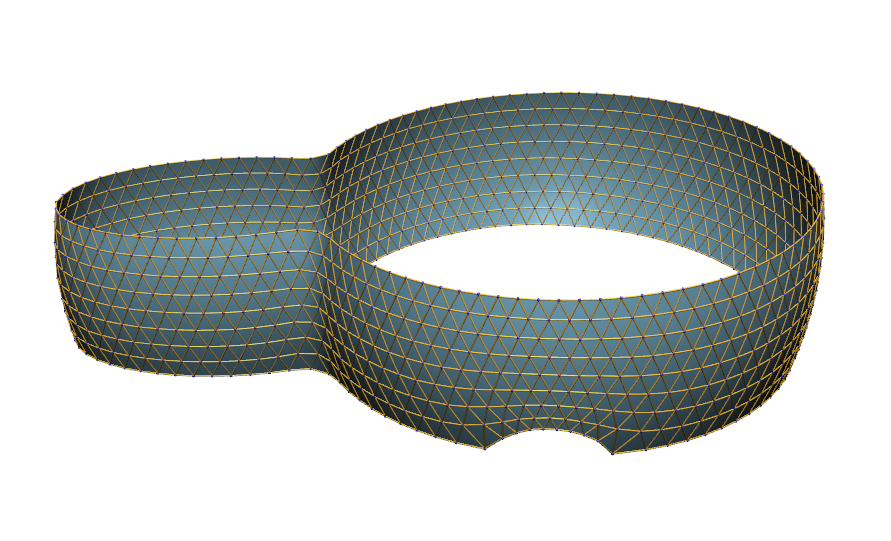
\includegraphics[width=.49\linewidth]{images/dc_entrance_cut.png}
  \caption{A conformal map onto a cylinder with three special vertices, that yields a more interesting panelization. It can be used to specify entrances, for example.}
  \label{fig:entrance}
\end{figure}

The effect of such angle conditions is a densification of the tiling
at the vertices with positive curvature. In the example shown in
Figure~\ref{fig:entrance} (right), we prescribed curvatures of
$\tfrac{2\pi}{3}$ and $-\tfrac{2\pi}{3}$, alternatingly. This yields a
nice zig-zag on the cylinder and in the plane.

\end{document}

%%% Local Variables: 
%%% mode: latex
%%% TeX-master: "article"
%%% End: 
